% LaTeX.tex
% Example of PROCEEDINGS PAPER of the 26th ABCM International Congress of Mechanical Engineering
% COBEM 2021 - ONLINE
% Based on the templates of COBEM2015, COBEM2017, and COBEM2019

\documentclass[10pt,fleqn,a4paper,twoside]{article}
\usepackage{abcm}
\usepackage{amsmath}
\usepackage{tikz}
\usepackage{float}
\usepackage{tikz}
\usetikzlibrary{patterns}
\usepackage{relsize}
\usetikzlibrary{shapes,arrows,arrows.meta,matrix}


\def\shortauthor{L. Marques and G. Anjos}
\def\shorttitle{A Blood Flow Numerical Simulation using FE Method for 2D-Axisymmetric Navier-Stokes Equation}



\begin{document}
\fphead
\hspace*{-2.5mm}\begin{tabular}{||p{\textwidth}}
\begin{center}
\vspace{-4mm}
\title{COB-2021-XXXX\\ 
BLOOD FLOW NUMERICAL SIMULATION USING FE METHOD FOR 2D-AXISYMMETRIC NAVIER-STOKES EQUATION} 
%
\end{center}
\authors{Leandro Marques} \\
\authors{Gustavo R. Anjos} \\
\institution{COPPE/Federal University of Rio de Janeiro - UFRJ, R. Horacio Macedo, 2030, Rio de Janeiro, Brazil}\\
\institution{marquesleandro.uerj@gmail.com and gustavo.rabello@coppe.ufrj.br} \\
\\
\abstract{\textbf{Abstract.} 
According to the World Health Organization, more people die annually from the cardiovascular disease (CVD) that from any other cause in the world. 
About 44\% of these deaths were due to coronary heart disease (CHD) in the United States.
For corrective treatments, the percutaneous transluminal coronary angioplasty (PTCA) is a effective minimally invasive procedure, where a small wire tube, called stents, is placed. 
This work aims to develop a FE code for 2D Axisymmetric Navier-Stokes with species transport equation using semi-Lagrangian scheme and to know how occurs the dynamics of blood flow in coronary artery with atherosclerosis and with stents struts placed.
The dynamics of blood flow in coronary artery and possible influence of stents struts with computational fluid dynamics (CFD) requires a robust numerical method to compute the solution of the differential equations in a relevant model. 
The equations that govern the dynamics of blood flow in a coronary artery were developed according to continuum media assumption. Thus, the universal conservation laws such as conservation of mass, conservation of momentum and conservation of species transport were used in an Eulerian context. 
The blood was modeled as single-phase, incompressible and newtonian fluid, the diffusion coefficient was considered as constant. 
The domain was discretized on an unstructured triangular mesh using the \textit{GMSH} open source. Due to coupling between velocity field and pressure field, the different triangular elements was used, where the linear element was used for pressure field and the \textit{MINI} element was used for velocity field.
The equations were discretized in space by Galerkin formulation and in time, the semi-Lagrangian scheme was used to discretized the material derivative using first order backward difference scheme.
The dynamics of blood flow and species transport in coronary artery was investigated in two complex geometry, where 
the first case is the \textit{Curved Channel with Stent}, 
where the atherosclerosis was modeled using a sinusoidal
equation to model 40\% of channel obstruction and
the second case is a \textit{Real Channel with Stent} 
and this geometry was obtained through an image processing in an
obstructed coronary artery due to the atherosclerosis.
In both case, the Reynolds number was calculated
using the blood parameters and the Schmidt number
was simulated for several cases.
}
\\
\\
\keywords{\textbf{Keywords:} Navier-Stokes, Axisymmetric, Finite Element Method, Semi-Lagrangian, Drug-Eluting Stent.}\\
\end{tabular}

%\section{INTRODUCTION}
%
%According to the World Health Organization, more people die annually from the cardiovascular disease (CVD) that from any other cause in the world. 
%%An estimated 17.9 million people died from CVD in 2016, representing 31\% of all global deaths. 
%About 44\% of these deaths were due to coronary heart disease (CHD) in the United States.
%For a corrective treatments, the percutaneous transluminal coronary angioplasty (PTCA) is a effective minimally invasive procedure, where a small wire tube, called stents, is placed. 
%This work aims to develop an FE code for 2D Axisymmetric Navier-Stokes Equation with species transport equation using semi-Lagrangian scheme and to know how occurs the dynamics of blood flow in coronary artery with atherosclerosis and with stents struts placed.
%
%\smallskip
%The dynamics of blood flow in coronary artery and possible influence of stents struts with computational fluid dynamics (CFD) requires a robust numerical method to compute the solution of the differential equations in a relevant model. 
%The equations that govern the dynamics of blood flow in a coronary artery were developed according to continuum media assumption. Thus, the universal conservation laws such as conservation of mass, conservation of momentum and conservation of species transport were used in an Eulerian context. 
%The blood was modeled as single-phase, incompressible and newtonian fluid, the diffusion coefficient was considered as constant. 
%The Navier-Stokes equation is shown with species transport equation in a Finite Element Method approach.
%
%\smallskip
%The domain was discretized on an unstructured triangular mesh using the \textit{GMSH} open source. Due to coupling between velocity field and pressure field, the different triangular elements was used, where the linear element was used for pressure field and the mini element was used for velocity field
%The equations were discretized in space by Galerkin formulation and in time, the semi-Lagrangian scheme was used to discretized the material derivative using first order backward difference scheme.
%
%\smallskip
%%The computational development was done in \textit{Python} language using object-oriented programming paradigm with the aim of reusability and further development.
%%The linear system of equations that comes from implementing the FEM is solved throught iterative method \textit{Conjugate Gradient Solver} available in the public library for scientific tools \textit{SciPy}. 
%%The code validation was made by comparison numerical solution and analytical solution of the \textit{Poiseuille flow}. The comparison of velocity field was done for lid-driven cavity flow with those shown by \citet{ghia1982} and \citet{marchi2009}.
%The dynamics of blood flow and species transport in coronary artery was investigated in two complex geometry, where 
%the first case is called the \textit{Curved Channel with Stent}, 
%the atherosclerosis was modeled using a sinusoidal
%equation to model 40\% of channel obstruction and
%the second case is a \textit{Real Channel with Stent} 
%and this geometry was obtained through an image processing in an
%obstructed coronary artery due to the atherosclerosis.
%In both case, the Reynolds number was calculated
%using the blood parameters and the Schmidt number
%was simulated for several cases.
%The simulation was shown using \textit{Paraview} open source.

%\section{MATHEMATICAL MODEL}
%A Finite Element Method approach is employed to analyse the dynamics of blood flow in coronary artery with atherosclerosis and possible influence of stents struts. 
%The governing equations were developed according to continuum media assumption. Thus, the universal conservation laws such as conservation of mass, conservation of momentum and conservation of species transport were used in an Eulerian context. 
%The blood was modeled as single-phase, incompressible and newtonian fluid, the diffusion coefficiente was considered as constant. The Navier-Stokes equation is shown with species transport equation in a two dimensional approach: 
%
%\begin{align}
%& \nabla \cdot \textbf{v} 
%= 0 \label{continuity}
%\\[10pt] 
%& \frac{\partial \textbf{v}}{\partial t} 
% + \textbf{v} \cdot \nabla \textbf{v}
% =
% - \nabla p
% + \frac{1}{Re} \nabla^{2} \textbf{v} \label{vorticity}
% \\[10pt] 
%& \frac{\partial e}{\partial t} 
% + \textbf{v} \cdot \nabla e
% =
% \frac{1}{ReSc} \nabla^{2} e \label{especie quimica}
%\end{align}
%
%
%\noindent
%where, 
%\textbf{v} is the material velocity field,
%\textit{p} is the pressure field,
%\textit{e} is the concentration field,
%$\nabla$ is the Del operator,
%\textit{Re} $= \rho uD/\mu$ is the Reynolds number,
%\textit{Sc} $= \nu / D$ is the Schmidt number and
%\textit{x} and \textit{y} are the spatial variables.
%
%\bigskip
%\noindent
%The boundaries conditions used were:
%
%\begin{itemize}
% \item \textit{inflow condition}:
% this condition is specified when an mass inflow is desired.
% For such a condition, the tangent velocity component
% is $u = u_{o}$ and the normal velocity component is $v=v_{o}$, 
% where the $u_{o} = 1.5\left[1-\left(y/R\right)^{2}\right]$ 
% and $v_{o}=0$.
%
% \item \textit{wall condition}:
% this condition is specified at wall boundaries (moving wall
% and noslip conditions).
% All the velocity components are specified with 
% the same wall velocity values.
%
% \item \textit{outflow condition}: 
% this condition represents a state where is close to a
% fully developed profile. 
% For this condition, the pressure field is set as $p=0$.
%
% \item \textit{free-slip condition}: 
% this condition is specified at the symmetric axis.
% The normal velocity component is null and the derivative of
% the tangent component is also null value.
%
% \item \textit{strut condition}: 
% this condition is used on the stent. The normal and tangential
% velocity components are specified with null value. 
% The concentration field is specified as $e=e_{o}$.
%\end{itemize}
%
%
%\subsection{Galerkin Method}
%The domain was discretized on an unstructured triangular mesh using the \textit{GMSH} open source. Due to coupling between velocity field and pressure field, differents triangular elements were used to velocity and pressure fields.
%The convective term of Eqs. \ref{vorticity}  and \ref{especie quimica} 
%will be replaced by material derivative for further time discretization
%using semi-Lagrangian Method. For spatial discretization of governing equations, 
%the Galerkin method was used, 
%resulting in the following matrix system:
%
%
%\vspace{-0.4cm}
%\begin{equation}
% D\textbf{v} = 0
%\end{equation}
%
%\vspace{-0.65cm}
%\begin{equation}
% M \frac{D \textbf{v}}{Dt} 
% + \frac{1}{\textit{Re}} \Big[ K_{xx} + K_{yy} \Big] \textbf{v}
% - Gp
% = 0 \label{vorticity matrix}
%\end{equation}
%
%\vspace{-0.65cm}
%\begin{equation}
% M \frac{De}{Dt} 
% + \frac{1}{\textit{ReSc}} \Big[ K_{xx} + K_{yy} \Big] e
% = 0 \label{concentration matrix}
%\end{equation}
%
%
%
%\noindent
%where,
%\textit{M} is mass matrix,
%\textit{D} is divergent matrix,
%\textit{G} is gradient matrix,
%\textit{$K_{xx}$} and
%\textit{$K_{yy}$} are stiffness matrix.
%
%
%
%\subsection{Semi-Lagrangian Scheme}
%The Semi-Lagrangian Scheme in centred difference was proposed by \cite{sawyer1963} for atmospheric flow numerical simulation using vorticity-advection equation, allowing to use large time steps without numerical instability. 
%However, because of a limited computer capability, the use of such methodology to model several fluid flow problems, with high order differences and fine mesh, came latter in the 1980's throught the work of \cite{robert1981} and \cite{pironneau1982}, where the semi-lagrangian scheme would be able to run models faster than the Eulerian scheme, besides be unconditionally stable and only symmetric linear systems to solve. 
%Basically, the semi-lagrangian scheme takes into account the fact that the Eulerian derivative is replaced by the material derivative, then it is discretized and computed along the trajectory characteristic:
%
%\vspace{-0.4cm}
%\begin{equation}
% \frac{D \textbf{v}}{D t} \approx
% \frac{\textbf{v}_{i}^{n+1} - \textbf{v}_{d}^{n}}{\Delta t}
%\end{equation}
%
%\noindent
%where, 
%$D\textbf{v}/Dt$ is material derivative of $\textbf{v}$ and
%the right-hand side equation is material derivative discretized using first order backward difference scheme.
%The variable $t$ is time, 
%$\textbf{v}_{i}^{n+1}$ is the velocity field calculated in current time step at the current node position and
%$\textbf{v}_{d}^{n}$ is the velocity field calculated in previous time step at the departure node position.
%
%\smallskip
%The departure node is found by solving equation $\mathbf{x}_{d}^{n} = \mathbf{x}_{i}^{n+1} - \mathbf{v} \Delta t$, using the initial condition $\mathbf{x}_{i}^{n+1} = \mathbf{x}(t^{n+1})$ as shown in Figure \ref{semi-lagrangian figure}a . 
%A algorithm must be used to find the element that the departure node be, then the velocity field in departure node ($\textbf{v}_{d}^{n}$) is calculed by barycenter coordinates interpolation between nodes of element found.
%As shown in Figure \ref{semi-lagrangian figure}b , three situations may occur depending on the trajectory: the first and the second situations are similar, differentiating only the trajectory length. 
%In the first situation, the departure node is inside near element from current node, while the second situation the departure node is inside far element from current node. 
%The third situation, the departure node is outside domain then the vorticity field in departure node receives the boundary condition value of nearest node to departure node.
%
%\vspace{-0.5cm}
%\begin{figure}[H]
%\begin{center}
%\begin{tikzpicture}[scale=4]
%
% % FIGURE A
% % grid
% \draw (0.5,0.7) -- (2.0,0.7);
% \draw (0.5,1.0) -- (2.0,1.0);
% \draw (0.5,1.2) -- (2.0,1.2);
%
% \draw (0.60,0.7) -- (0.64,1.0) -- (0.60,1.2);
% \draw (1.20,0.7) -- (1.12,1.0) -- (1.10,1.2);
% \draw (1.54,0.7) -- (1.64,1.0) -- (1.50,1.2);
% \draw (1.85,0.7) -- (1.90,1.0) -- (1.90,1.2);
%
%
%
% % material points
% \draw[dashed,-stealth] (1.12,1.0) -- (0.85,0.75);
% \node[rectangle, fill=white, draw, inner sep=0pt, minimum size=9.4pt] at (0.8,0.7) {};
% \node[rectangle, fill=white, draw, inner sep=0pt, minimum size=9.4pt] at (1.12,1.0) {};
% 
%
% % nodes
% \node[circle, fill=black, inner sep=0pt, minimum size=5.2pt] at (0.60,0.7) {};
% \node[circle, fill=black, inner sep=0pt, minimum size=5.2pt] at (1.20,0.7) {};
% \node[circle, fill=black, inner sep=0pt, minimum size=5.2pt] at (1.54,0.7) {};
% \node[circle, fill=black, inner sep=0pt, minimum size=5.2pt] at (1.85,0.7) {};
%
% \node[circle, fill=black, inner sep=0pt, minimum size=5.2pt] at (0.64,1.0) {};
% \node[circle, fill=black, inner sep=0pt, minimum size=5.2pt] at (1.12,1.0) {};
% \node[circle, fill=black, inner sep=0pt, minimum size=5.2pt] at (1.64,1.0) {};
% \node[circle, fill=black, inner sep=0pt, minimum size=5.2pt] at (1.90,1.0) {};
%
% \node[circle, fill=black, inner sep=0pt, minimum size=5.2pt] at (0.60,1.2) {};
% \node[circle, fill=black, inner sep=0pt, minimum size=5.2pt] at (1.10,1.2) {};
% \node[circle, fill=black, inner sep=0pt, minimum size=5.2pt] at (1.50,1.2) {};
% \node[circle, fill=black, inner sep=0pt, minimum size=5.2pt] at (1.90,1.2) {};
%
%
% % legend
% \node[draw=none, scale=1.0] at (0.80,0.82) {\small $\mathbf{x}_{d}$};
% \node[draw=none, scale=1.0] at (1.22,0.88) {\small $\mathbf{x}_{i}$};
%
% \node[draw=none, scale=1.0] at (2.10,0.70) {\small $t^{n}$};
% \node[draw=none, scale=1.0] at (2.15,1.00) {\small $t^{n+1}$};
% \node[draw=none, scale=1.0] at (2.15,1.20) {\small $t^{n+2}$};
%
% \node[draw=none, scale=1.0] at (0.60,0.55) {\small $\mathbf{x}_{i-1}$};
% \node[draw=none, scale=1.0] at (1.22,0.55) {\small $\mathbf{x}_{i}$};
% \node[draw=none, scale=1.0] at (1.64,0.55) {\small $\mathbf{x}_{i+1}$};
%
%
% % -------------------------------------------------------------------
% % FIGURE B
% % boundary 
% \draw (2.5,1.6) -- (4.0,1.6);
% \draw (2.5,1.6) -- (2.5,0.5);
% \draw (2.5,0.5) -- (4.0,0.5);
%
% % nodes
% \coordinate (A) at (2.500,0.5000) {};
% \coordinate (B) at (2.500,0.8667) {};
% \coordinate (C) at (2.500,1.2330) {};
% \coordinate (D) at (2.500,1.6000) {};
% \coordinate (E) at (2.733,0.6830) {};
% \coordinate (F) at (2.833,1.0500) {};
% \coordinate (G) at (2.733,1.4160) {};
% \coordinate (H) at (3.000,1.6000) {};
% \coordinate (I) at (3.066,0.5000) {};
% \coordinate (J) at (3.166,0.8660) {};
% \coordinate (K) at (3.150,1.3330) {};
% \coordinate (L) at (3.333,1.6000) {};
% \coordinate (M) at (3.500,0.5000) {};
% \coordinate (N) at (3.333,0.6830) {};
% \coordinate (O) at (3.400,1.0000) {};
% \coordinate (P) at (3.500,1.2300) {};
%
% % elements
% \draw (A) -- (E) -- (B) -- cycle;
% \draw (A) -- (I) -- (E) -- cycle;
% \draw (E) -- (J) -- (F) -- cycle;
% \draw (E) -- (F) -- (B) -- cycle;
% \draw (B) -- (F) -- (C) -- cycle;
% \draw (J) -- (K) -- (F) -- cycle;
% \draw (F) -- (K) -- (G) -- cycle;
% \draw (C) -- (F) -- (G) -- cycle;
% \draw (C) -- (G) -- (D) -- cycle;
% \draw (G) -- (H) -- (D) -- cycle;
% \draw (I) -- (N) -- (J) -- cycle;
% \draw (I) -- (M) -- (N) -- cycle;
% \draw (N) -- (O) -- (J) -- cycle;
% \draw (J) -- (O) -- (K) -- cycle;
% \draw (P) -- (L) -- (K) -- cycle;
% \draw (K) -- (L) -- (H) -- cycle;
% \draw (O) -- (P) -- (K) -- cycle;
% \draw[red,line width=0.04cm] (I) -- (J) -- (E) -- cycle;
% \draw[red,line width=0.04cm] (B) -- (C);
% \draw[red,line width=0.04cm] (G) -- (K) -- (H) -- cycle;
% 
%
% % draw nodes
% \node[circle, fill=black, inner sep=0pt, minimum size=5.2pt] at (A) {};
% \node[circle, fill=black, inner sep=0pt, minimum size=5.2pt] at (B) {};
% \node[circle, fill=black, inner sep=0pt, minimum size=5.2pt] at (C) {};
% \node[circle, fill=black, inner sep=0pt, minimum size=5.2pt] at (D) {};
% \node[circle, fill=black, inner sep=0pt, minimum size=5.2pt] at (E) {};
% \node[circle, fill=black, inner sep=0pt, minimum size=5.2pt] at (F) {};
% \node[circle, fill=black, inner sep=0pt, minimum size=5.2pt] at (G) {};
% \node[circle, fill=black, inner sep=0pt, minimum size=5.2pt] at (H) {};
% \node[circle, fill=black, inner sep=0pt, minimum size=5.2pt] at (I) {};
% \node[circle, fill=black, inner sep=0pt, minimum size=5.2pt] at (J) {};
% \node[circle, fill=black, inner sep=0pt, minimum size=5.2pt] at (K) {};
% \node[circle, fill=black, inner sep=0pt, minimum size=5.2pt] at (L) {};
% \node[circle, fill=black, inner sep=0pt, minimum size=5.2pt] at (M) {};
% \node[circle, fill=black, inner sep=0pt, minimum size=5.2pt] at (N) {};
% \node[circle, fill=black, inner sep=0pt, minimum size=5.2pt] at (O) {};
% \node[circle, fill=black, inner sep=0pt, minimum size=5.2pt] at (P) {};
%
%
% % arrow
% \draw[dashed,line width=0.03cm,-stealth]  (2.95,0.65) -- (J) ;
% \draw[dashed,line width=0.03cm,-stealth]  (2.90,1.45) -- (J) ;
% \draw[dashed,line width=0.03cm,-stealth]  (2.4,1.05)  -- (J) ;
%
% \node[circle, fill=black, inner sep=0pt, minimum size=5.2pt] at (J) {};
%
% % departure nodes
% \node[circle, fill=white, draw, inner sep=0pt, minimum size=5.2pt] at (2.95,0.65) {};
% \node[circle, fill=white, draw, inner sep=0pt, minimum size=5.2pt] at (2.90,1.45) {};
% \node[circle, fill=white, draw, inner sep=0pt, minimum size=5.2pt] at (2.4,1.05) {};
%
%
% 
% % legend
% \node[draw=none, scale=0.9] at (3.23,0.97) {\small $\textbf{v}_{i}$};
% 
% \node[draw=none, scale=0.9] at (3.05,0.64) {$1$};
% \node[draw=none, scale=0.9] at (3.00,1.45) {$2$};
% \node[draw=none, scale=0.9] at (2.4,1.15) {$3$};
%
% \node[draw=none, scale=1.0] at (3.7,1.0) {\small $domain$};
% \node[draw=none, scale=1.0] at (3.8,1.65) {\small $boundary$};
%
%
%
% \node[draw=none, scale=0.8] at (1.23,0.3) {\large (a)};
% \node[draw=none, scale=0.8] at (3.25,0.3) {\large (b)};
%
%\end{tikzpicture}
%\end{center}
%\caption{In (a), an one-dimensional space scheme
% where the departure node $x_{d}$ is found by integrating the 
%mesh backward time. In (b), a two-dimensional space scheme
%where three situations may occur in searching procedure.}
%\label{semi-lagrangian figure}
%\end{figure}
%
%\medskip
%The triangular element with linear interpolation was used
%for the pressure field and a modified cubic element 
%(2D MINI) was used
%for the velocity field, 
%in order to respect the Babuska-Brezzi restriction
%\cite{babuska1971}\cite{brezzi1974}.
%These elements consists in three nodes in the vertices
%and one node in the baricentric for MINI element case.
%The elementary matrices of 
%this element are calculated using the Gaussian Quadrature, 
%whose parameters can be found in the literature \cite{cowper1973}. 
%These elements are represented by:
%
%\begin{figure}[H]
%\begin{center}
%\vspace{-0.5cm}
%\begin{tikzpicture}[scale=3] 
% \draw (0,0) -- (1,0) -- (0.5,1) -- cycle;
% \node[circle, fill=black, inner sep=0pt, minimum size=5pt,label=below left:{1}] at (0,0) {};
% \node[circle, fill=black, inner sep=0pt, minimum size=5pt,label=below right:{2}] at (1,0) {};
% \node[circle, fill=black, inner sep=0pt, minimum size=5pt,label=above:{3}] at (0.5,1) {};
% \node[circle, fill=black, inner sep=0pt, minimum size=5pt,label=below:{4}] at (0.5,0.33) {};
% \node[draw, circle, thick, minimum size=7pt,label=below left:{}] at (0,0) {};
% \node[draw, circle, thick, minimum size=7pt,label=below left:{}] at (1,0) {};
% \node[draw, circle, thick, minimum size=7pt,label=below left:{}] at (0.5,1) {};
%
% \node[circle, fill=black, inner sep=0pt, minimum size=5pt,label=right left:{velocity nodes}] at (1.5,0.5) {};
% \node[circle, draw, thick, inner sep=0pt, minimum size=7pt,label=right left:{pressure nodes}] at (1.5,0.3) {};
%
% \node[draw=none, align=left, scale=1.2] at (3.2,0.4)
%                                               {$N_1 = L_1 - 9L_1L_2L_3$\\
%                                                $N_2 = L_2 - 9L_1L_2L_3$\\
%                                                $N_3 = L_3 - 9L_1L_2L_3$\\
%                                                $N_4 = 27L_1L_2L_3$};
%
%
%
%\end{tikzpicture}
%\end{center}
%\caption{
%The linear triangle finite element
%for pressure field and
%the MINI element for velocity field.
%The
%$L_1$,
%$L_2$ and
%$L_3$
%are the linear combination
%of the triangle area
%coordinates and
%$N_1$,
%$N_2$,
%$N_3$ and
%$N_4$
%are the resulting shape functions.
%}
%
%\end{figure}
%
%\noindent
%where, 
%a linear combination of the area
%coordinates
%$L_1$,
%$L_2$ and
%$L_3$ 
%generates the shape functions
%$N_1$ to $N_4$. 
%The pressure $p$ and
%concentration $e$ fields
%are evaluated and computed at vertice nodes,
%while the velocity field $\textbf{v}$
%is evaluated and computed at all nodes.
%Thus, we present the final version of
%the discrete matrix form of the
%dimensionless governing equations
%used in this work:
%
%
%\vspace{-0.4cm}
%\begin{equation}
% D\textbf{v}_{i}^{n+1}=0
%\end{equation}
%
%\vspace{-0.45cm}
%\begin{equation}
% \left[
% \frac{M}{\Delta t} 
% + \frac{1}{\textit{Re}} \left[ K_{xx} + K_{yy} \right]
% \right] 
% \textbf{v}^{n+1}_{i}
% - Gp^{n+1}
% = \frac{M}{\Delta t} \textbf{v}^{n}_{d}
%\end{equation}
%
%\vspace{-0.55cm}
%\begin{equation}
% \left[
% \frac{M}{\Delta t} 
% + \frac{1}{\textit{ReSc}} \left[ K_{xx} + K_{yy} \right]
% \right] 
% e^{n+1}_{i}
% = \frac{M}{\Delta t} e^{n}_{d}
%\end{equation}
%
%
%
%\section{RESULTS AND DISCUSSION}
%
%%The computational development was done in \textit{Python} language using object-oriented programming paradigm with the aim of reusability and further development.
%%The linear system of equations that come from implementing the FEM is solved throught iterative method \textit{Conjugate Gradient Solver} available in the public library for scientific tools \textit{SciPy} maintained by \citet{scipy}.
%%Some results of simulations are shown to demonstrate its capability of using unstructured triangular meshes on various geometries and combination of geometries. 
%%Numerical results are given for several cases of blood flows in artery when $Sc=10$.
%%The post-processing was performed by open source software \textit{PARAVIEW} proposed by \citet{paraview}.
%
%In this section, we will present the results obtained from 
%several cases with the numerical simulation of the Navier Stokes 
%equation 
%with the species transport equation, 
%where we have incompressible 
%and monophase two-dimensional flow for all cases
%in an Eulerian context
%using the semi-Lagrangian Method. 
%In all simulations, the computational mesh velocity is
%calculated using only the Laplacian smoothing velocity.
%
%\smallskip
%Initially,
%the \textit {Poiseuille Symmetric} is shown, where the 
%free slip condition is applied on the axis of symmetry and no-slip condition is applied in the top wall. 
%Lastly, the results of numerical simulations for 
%blood flow in a coronary artery are presented. 
%The lumen radius of the coronary artery used was $R=0.0015m$, 
%the viscosity used was $\mu=0.0035Pa.s$ and the density used was
%$\rho=1060kg/m^3$ as suggested \cite{bozsak2014}. 
%According to \cite{kessler1998}, 
%the blood velocity in the coronary artery 
%is $u=12cm/s$. Thus, the Reynolds number used will be 
%$Re=54.5$. 
%
%\medskip
%The Navier-Stokes equation is used with 
%the species transport equation for two geometries proposed 
%by \cite{wang2017}, however modified to 
%cartesian coordinates as shown in Fig. \ref{coronary artery geo} . 
%In the Fig. (a), the numerical 
%simulation for the coronary artery with atherosclerosis 
%and a drug-eluting stent in a curved channel model 
%is presented for 
%\textit{Schmidt} number equal to $10$. 
%In the Fig. (b), the real coronary 
%artery with atherosclerosis and a drug-eluting stent is also 
%simulated with the same \textit{Schmidt} number 
%as in the previous section.
%Due to symmetry, only half of the domain is shown. 
%The simulation was visualized using the \textit{Paraview} open-source 
%software proposed by \cite{paraview}.
%
%
%\begin{figure}[H]
%     \begin{center}
%     \begin{minipage}{.45\linewidth}
%     \begin{center}
%      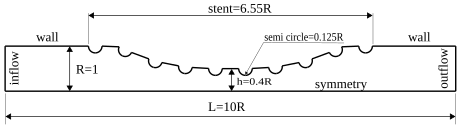
\includegraphics[scale=0.45]{./figure/CurvedStrut.png}\\
%     (a) Curved Channel
%     \end{center}
%     \end{minipage}%
%     \begin{minipage}{.45\linewidth}
%     \begin{center}
%      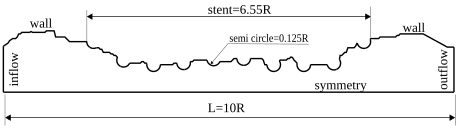
\includegraphics[scale=0.45]{./figure/RealStrut.png}\\
%     (b) Real Channel
%     \end{center}
%     \end{minipage}\\[3mm]
%     \end{center}
%     \label{coronary artery geo}
%     \caption{Non-dimensional domain for the blood flow in coronary artery
%     The radius used was $R=1$ and and the lumen length was $L=10R$ as proposed by \cite{wang2017}}
%\end{figure}
%
%
%
%\section{PRELIMINARY CONCLUSION}
%In this work, a numerial code for Navier-Stokes equation according to 
%with species
%transport equation was developed using an FE approach.
%The semi-Lagrangian scheme was used to discretized the material derivative
%using first order backward difference scheme and the numerical oscillations
%were not seen for moderate to high Schmidt number.
%
%\smallskip
%%The dynamics of blood flow was shown to a coronary artery with atherosclerosis and
%%drug-eluting stent placed.
%%It is possible to observe in the Fig. \ref{conc field curved stent sc 10}  that
%%the concentration field
%%is more dispersed at the end of the curved channel due to
%%the sense of the blood flow. It is possible that the
%%drug concentration diffused affects the density and viscosity of the blood
%%and consequently the Reynolds number. Thefore, the velocity field would
%%also be affected. However, this influence is not considered in this work.
%
%
%
%\section{ACKNOWLEDGEMENTS}
%This optional section must be placed before the list of references.
%
%\section{REFERENCES} 
%\label{Sec:references}
%
%\bibliographystyle{abcm}
%\renewcommand{\refname}{}
%\bibliography{references}
%
%
%
%\section{RESPONSIBILITY NOTICE}
%The following text, properly adapted to the number of authors, must be included in the last section of the paper:
%
%The author(s) is (are) solely responsible for the printed material included in this paper.
%
\end{document}
